\documentclass[a4paper,12pt]{article}
\usepackage{xcolor}
\usepackage{amsmath,amsfonts,amssymb}
\usepackage{geometry}
\usepackage{fancyhdr}
\usepackage{graphicx}
\usepackage{titlesec}
\usepackage{tikz}
\usepackage{booktabs}
\usepackage{array}
\usetikzlibrary{shadows}
\usepackage{tcolorbox}
\usepackage{float}
\usepackage{lipsum}
\usepackage{mdframed}
\usepackage{pagecolor}
\usepackage{mathpazo}   % Palatino font (serif)
\usepackage{microtype}  % Better typography
\usepackage{url}

\setlength{\parindent}{0pt}

% Page background color
\pagecolor{gray!10!white}

% Geometry settings
\geometry{margin=0.5in}
\pagestyle{fancy}
\fancyhf{}

% Fancy header and footer
\fancyhead[C]{\textbf{\color{blue!80}Onions: Are they always tasty?}}
% \fancyhead[R]{\color{blue!80}Saksham Rathi}
\fancyfoot[C]{\thepage}

% Custom Section Color and Format with Sans-serif font
\titleformat{\section}
{\sffamily\color{purple!90!black}\normalfont\Large\bfseries}
{\thesection}{1em}{}

% Custom subsection format
\titleformat{\subsection}
{\sffamily\color{cyan!80!black}\normalfont\large\bfseries}
{\thesubsection}{1em}{}

% Stylish Title with TikZ (Enhanced with gradient)
\newcommand{\cooltitle}[1]{%
\begin{tikzpicture}
\node[fill=blue!20,rounded corners=10pt,inner sep=12pt, drop shadow, top color=blue!50, bottom color=blue!30] (box)
{\Huge \bfseries \color{black} #1};
\end{tikzpicture}
}
\usepackage{float} % Add this package

\newenvironment{solution}[2][]{%
\begin{mdframed}[linecolor=blue!70!black, linewidth=2pt, roundcorner=10pt, backgroundcolor=yellow!10!white, skipabove=12pt, skipbelow=12pt]%
	\textbf{\large #2}
	\par\noindent\rule{\textwidth}{0.4pt}
}{
\end{mdframed}
}

% Document title
\title{\cooltitle{CS790 Assignment 3} \\
\LARGE \textbf{Onions: Are they always tasty?} \\
Report}
\author{{\bf Kavya Gupta (22B1053)} \\
\small Department of Computer Science, \\
Indian Institute of Technology Bombay \\}
\date{}

\begin{document}
\maketitle

\begin{solution}{Task 1}
    \begin{itemize}
        \item Coded in Python using the \texttt{stem} library in \texttt{make\_4-hop\_circuit.py}.
        \item Accessed \texttt{tor} easily (with suitable configurations) with \texttt{stem.process}. Used \texttt{pycurl} to send a web request (I did for \url{https://check.torproject.org}).
        \item Randomly selected 1 entry, 1 exit and 2 middle nodes and built the circuit with the library.
        \item From the above url, I got a response that we are indeed connecting via \texttt{Tor} but not via \texttt{Tor Browser}, showing success of the connection.
        \item Used the \texttt{nyx} program to confirm the circuit ID with the destination IP address, both of which matched.
        \begin{enumerate}
            \item Circuit and its ID (which is 9 as shown in Figure \ref{task_1}) printed by my Python script matched with those in \texttt{nyx}.
            \item The destination IP (which is \texttt{204.137.14.106} as shown in Figure \ref{nyx}) shown in \texttt{nyx} for that circuit ID matched with the IP returned by the above url (which claimed it to be \textit{my} IP from its perspective).
        \end{enumerate}
    \end{itemize}
    \begin{figure}[H]
        \centering
        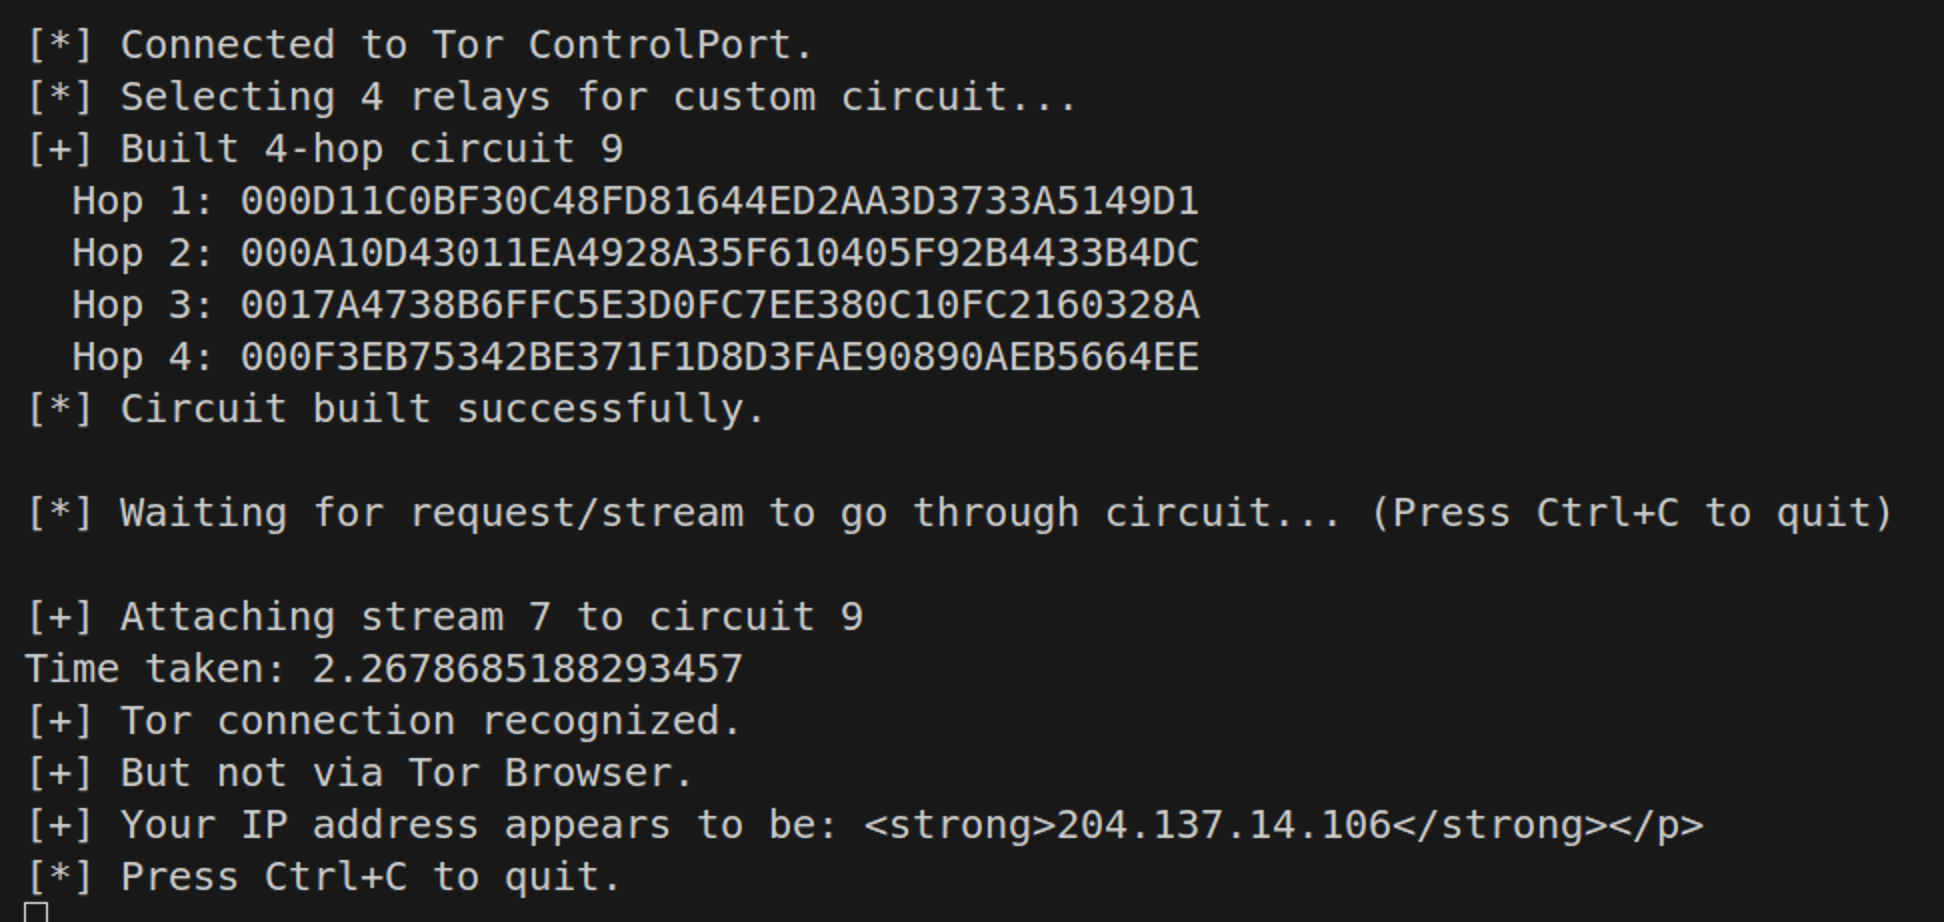
\includegraphics[width=0.6\textwidth]{../Task 1.png}
        \caption{Output of the Python Script}
        \label{task_1}
    \end{figure}
    \begin{figure}[H]
        \centering
        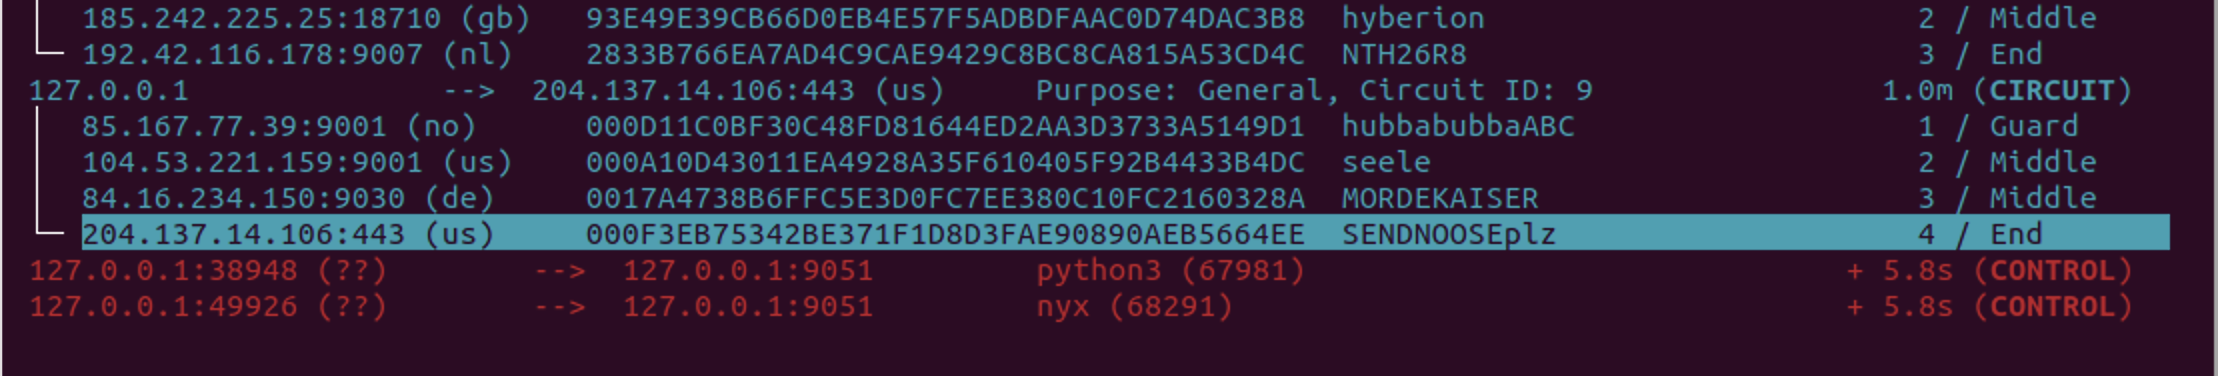
\includegraphics[width=0.75\textwidth]{../Task 1 Nyx.png}
        \caption{Output of the Nyx program}
        \label{nyx}
    \end{figure}
\end{solution}

\begin{solution}{Task 2}
    \begin{itemize}
        \item Coded in \texttt{circuit\_selector.py} but used as \texttt{python3 make\_4-hop\_circuit.py --task 2}.
        \item Made a function \texttt{get\_path(num\_hops)} that returns a valid ``\texttt{num\_hops}''-hops TOR relay path.
        \item Fetches the latest consensus and server descriptor files and parses them using \texttt{parse\_file()}.
        \item Followed the rules mentioned in section 2.2 of \url{https://github.com/torproject/torspec/blob/main/path-spec.txt}:-
        \begin{enumerate}
            \item Unique nodes
            \item Picked in the order of first Exit, then Guard and finally middle node(s)
            \item Not two nodes in the same family (found in \texttt{FAMILY} attribute of the server descriptors)
            \item Not two nodes in the same \texttt{/16} network
            \item Among the viable candidates, the winner was picked randomly with probability proportional to their \texttt{BANDWIDTH} attribute
        \end{enumerate}
        \item As can be seen in Figure \ref{task-2}, the circuit ID and destination IP matches for the Python script and \texttt{nyx}, hence proving the correctness.
    \end{itemize}
    \begin{figure}[H]
        \centering
        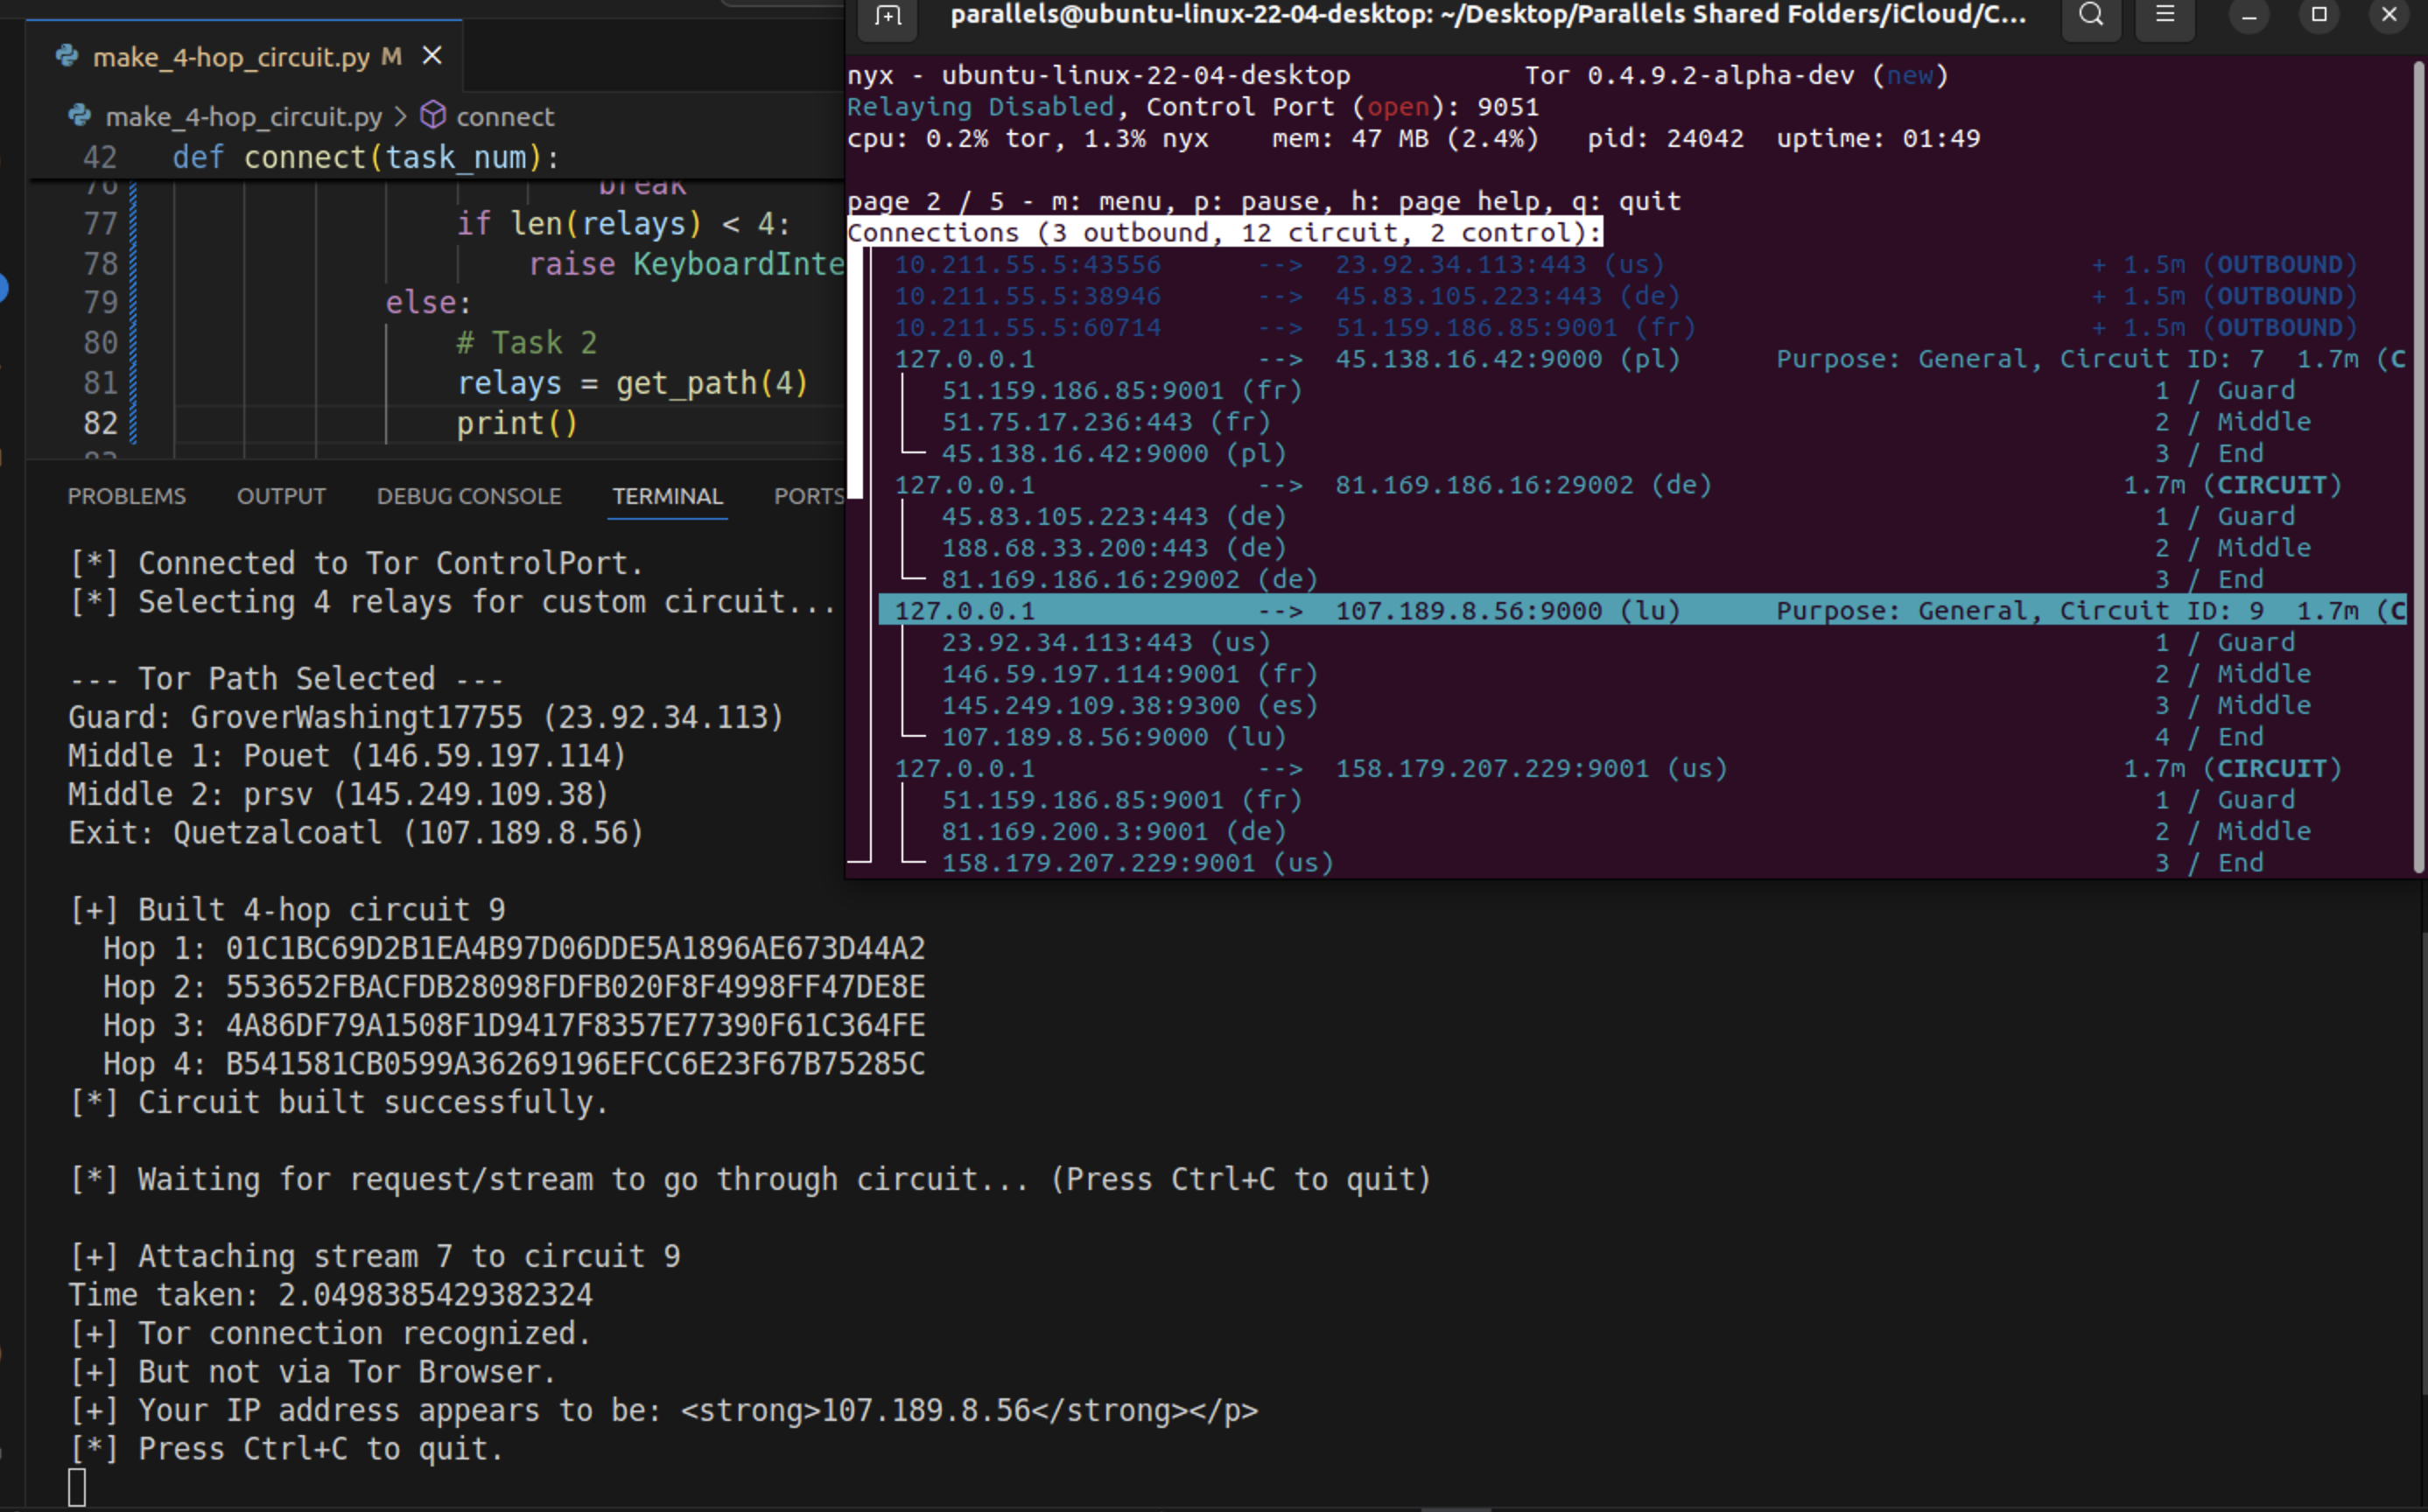
\includegraphics[width=0.75\textwidth]{../Task 2.png}
        \caption{Outputs of the Python script and Nyx program side-by-side}
        \label{task-2}
    \end{figure}
\end{solution}

\end{document}